\documentclass{article}
\usepackage{tikz}
\usepackage[utf8]{inputenc}
\usepackage[english]{babel}
\usepackage{amsfonts}
\usepackage{amsthm}
\usepackage{amsmath}
\usepackage{amssymb}

\newtheorem{theorem}{Theorem}
\newtheorem{es}{Examples}

\newcommand{\inter}[1]{int(#1)}

\title{MATC27 Assignment 4}
\author{Anmol Bhullar - 1002678140}

\begin{document}
    \maketitle
    \textbf{P1.}\\ 
    In order to show $d_U$ is a metric on $U$, we have to that for all $x,y,z\in U$ the following conditions hold: (i) $d_U(x,y)\geq 0$ (ii) $d_U(x,y)=0
    \leftrightarrow x=y$ (iii) $d_U(x,y)=d_U(y,x)$ and (iv) $d_U(x,z)\leq d_U(x,y)+d_U(y,z)$\\
    (i) It is clear that $|\frac{1}{d(x,U^c)} - \frac{1}{d(y,U^c)}|\geq 0$. Furthermore, since $d(x,y)$ is a metric on $X$, then since $U\subseteq X$,
    we have that $x,y\in X$ so that $d(x,y)\geq 0$ by (i). Thus, it follows that $0 + 0 \leq d(x,y) + |\frac{1}{d(x,U^c)}-\frac{1}{d(y,U^c)}|$
    so that $d(x,y)\geq 0$ as wanted.\\
    (ii) Assume $x=y$, we show $d_U(x,y)=0$. Note $d(x,y)=0$ since $d$ is a metric space. Furthermore, $|\frac{1}{d(x,U^c)}-\frac{1}{d(y,U^c)}| = 
    |\frac{1}{d(x,U^c)} - \frac{1}{d((x),U^c)} = 0$. Thus, it follows that $d_U(x,y) = 0$. Now, assume $d_U(x,y)=0$, we show $x=y$ and show $d_U(x,y)=0$.
    Somewhat similar to as before, we know $x=y$ implies $d(x,y)=0$ since $d$ is a metric. This implies that $|\frac{1}{d(x,U^C)}-\frac{1}{d(y,U^c)}|=0$
    which implies that $d(x,U^c)=d(y,U^c)$ so we have that: inf$\{d(x,a):a\in A\}$ = inf$\{d(y,a):a\in A\}$. Note:
    \begin{align*}
        \text{inf}\{d(x,a): a\in A\} - \text{inf}\{d(y,a): a\in A\} = 0 \\
        \text{inf}\{d(x,a) - d(y,a): a\in A\} = 0
    \end{align*}
    (iii) Note $d(x,y) = d(y,x)$ since $d$ is a metric space. Also, since $|a-b| = |b-a|$ for all real numbers $a$ and $b$, we obtain the fact:
    $|\frac{1}{d(x,U^c)} - \frac{1}{d(y,U^c)}|$. Combining these two results, we obtain that $d(x,y) + |\frac{1}{d(x,U^c)} - \frac{1}{d(y,U^c)}| = d(y,x) +
    |\frac{1}{d(y,U^c)} - \frac{1}{d(x,U^c)}|$. Thus, $d_U(x,y) = d_U(y,x)$ as wanted.\\
    (iv) Note since $d$ is a metric, then $d(x,z)\leq d(x,y) + d(y,z)$. Note that $d$ is a metric, then $d(x,U^c)$ is a real number for
    all $x\in X$ and we can apply the triangle inequality to all real numbers. Thus, consider the following:
    \begin{align*}
        &|\frac{1}{d(x,U^c)} - \frac{1}{d(y,U^c)}| + |\frac{1}{d(y,U^c)} - \frac{1}{d(z,U^c)}| \\
        &\geq |(\frac{1}{d(x,U^c)} - \frac{1}{d(y,U^c)}) + (\frac{1}{d(y,U^c)} - \frac{1}{z,U^c})|\qquad\text{triangle inequality}\\
        &= |\frac{1}{d(x,U^c)} - \frac{1}{d(z,U^c)}|
    \end{align*}
    Combining these two results, we get that $d_U(x,z)\leq d_U(x,y)+d_U(y,z)$ as wanted.\\
    Since conditions (i)..(iv) all hold for all $x,y,z\in U$, we obtain the result that $d_U$ is a metric on $U$.\\

    \textbf{P2}.\\
    The discrete metric $d_1$ on $\mathbb{R}^2$ is defined by $d_1(x,y)=0$ if $x=y$ and $d_1(x,y)=1$ if $x\neq y$. Thus, it is easy to see that
    $B_{d_1}(0,1) = \{0\}$. This would look like:
    \begin{center}
    \begin{tikzpicture}[scale=1]
        \draw (-1.5,0) -- (1.5,0);
        \draw (0,-1.5) -- (0,1.5);
        \draw (0,0) circle[radius=2pt];
        \fill (0,0) circle[radius=2pt];

        \foreach \x in {-1,0,1}
            \draw (\x cm, 1pt) -- (\x cm, -1pt) node[anchor=north] {$\x$};
        \foreach \y in {-1,1}
            \draw (1pt, \y cm) -- (-1pt, \y cm) node[anchor=east] {$\y$};
    \end{tikzpicture}
    \end{center}
    We know that the euclidean distance is the shortest distance between two points, thus the ball $B_{d_2}(0,1)$ is the set of points that
    are less than 1 "unit" (or more appropriately in this instance) epsilon from $0$. This naturally gives us the circle as seen below:
    \begin{center}
        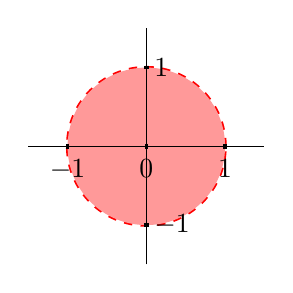
\begin{tikzpicture}
            \draw[red,very thick,dashed] (0,0) circle (1cm);
            \fill[red!40!white] (0,0) circle (1cm);
            \draw[step=.5cm,gray,very thin] (-1.4,1.4) grid (-1.4,1.4);
            \draw (-1.5,0) -- (1.5,0);
            \draw (0,-1.5) -- (0,1.5);
            \foreach \x in {-1,0,1}
                \draw[very thick] (\x cm, 1pt) -- (\x cm, -1pt) node[anchor=north] {$\x$};
            \foreach \y in {-1,1}
                \draw[very thick] (1pt, \y cm) -- (-1pt, \y cm) node[anchor=west] {$\y$};
        \end{tikzpicture}
    \end{center}
    Since $d_3((x_1,y_1),(x_2,y_2)) = |x_1-x_2|+|y_1-y_2|$, then if we set $(x_2,y_2) = (0,0)$, we get $d_3((x_1,y_1),(0,0)) = |x_1|+|y_1|$. Thus,
    $B_{d_3}(0,1) = \{(x,y): |x|+|y|<1\}$. From this, we can see that some of the boundary points of this set are the points $(0,1),(0,-1),(1,0),(-1,0)$ and
    $(0.5,0.5),(-0.5,-0.5),(-0.5,0.5),(0.5,-0.5)$. Extrapolating from these points, we can see that $B_{d_3}(0,1)$ is representated by the image:
    \begin{center}
        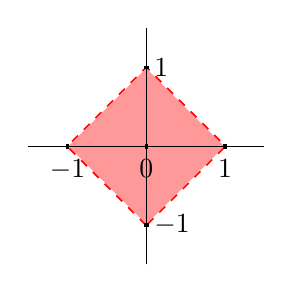
\begin{tikzpicture}
            \draw[red,very thick,dashed,shift={(0cm,0cm)},rotate=45] (-0.7,-0.7) rectangle (0.7,0.7);
            \fill[red!40!white,rotate=45] (-0.7,-0.7) rectangle (0.7,0.7);
            \draw[step=.5cm,gray,very thin] (-1.4,1.4) grid (-1.4,1.4);
            \draw (-1.5,0) -- (1.5,0);
            \draw (0,-1.5) -- (0,1.5);
            \foreach \x in {-1,0,1}
                \draw[very thick] (\x cm, 1pt) -- (\x cm, -1pt) node[anchor=north] {$\x$};
            \foreach \y in {-1,1}
                \draw[very thick] (1pt, \y cm) -- (-1pt, \y cm) node[anchor=west] {$\y$};
        \end{tikzpicture}
    \end{center}
    Observing the "rule" for $d_4$, we immediately see that $B_{d_4}(0,1) = \{(x,y):\:\text{max}\{|x|,|y|\}<1\}$. Thus, $B_{d_4}(0,1)$ contains
    any points contained by the lines $x=1,x=-1,y=1,y=-1$. This is given by the square as shown below:
    \begin{center}
        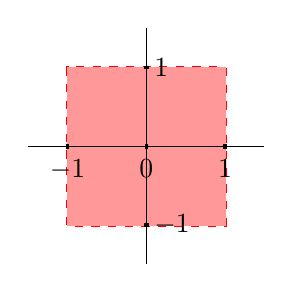
\begin{tikzpicture}
            \draw[red,very thick,dashed] (-1,-1) rectangle (1,1);
            \filldraw[red!40!white] (-1,-1) rectangle (1,1);
            \draw[step=.5cm,gray,very thin] (-1.4,1.4) grid (-1.4,1.4);
            \draw (-1.5,0) -- (1.5,0);
            \draw (0,-1.5) -- (0,1.5);
            \foreach \x in {-1,0,1}
                \draw[very thick] (\x cm, 1pt) -- (\x cm, -1pt) node[anchor=north] {$\x$};
            \foreach \y in {-1,1}
                \draw[very thick] (1pt, \y cm) -- (-1pt, \y cm) node[anchor=west] {$\y$};
        \end{tikzpicture}
    \end{center}

    \textbf{P3}.\\
    Let $X$ be a finite (cardinality) set equipped with a metric $d$. We show $d$ induces the discrete topology. Index $X$ so that $X = \{x_1,\hdots,x_k\}$ for
    some $k\in\mathbb{N}$. Then fix $x_i$ for some $1\leq i\leq k$ and let $\rho = $min$\{d(x_i,x_j): x_j\in X, x_j\neq x_i\}$. By property (ii) (defined in 
    \textbf{P1}) of a metric space, we know $\rho\neq 0$. Thus, choose $0<\xi<\rho$ for some $\xi\in\mathbb{R}$. Then, by construction of $\xi$, we 
    know that $B_{d}(x_i,\xi) = \{x_i\}$ so that $\{x_i\}$ is open in $\tau_{(X,d)}$. 
    Since $x_i$ is arbitrary, we can repeat this process again for some other $x_i$ to obtain that all singletons are open 
    in $\tau_{(X,d)}$ which implies that $\tau_{(X,d)}$ is the discrete topology (Lecture Exercises A1 \#4).\hfill$\blacksquare$\\

    \textbf{P4}.\\
    Let $f: X \to Y$ be a continouous function between topological spaces $X$ and $Y$ that are induced by the metrics $d$ and $d_Y$ respectively. We want to show
    $f_A: A \to Y$ is continouous if $A\subseteq X$ is a topological space metrized by the subspace metric $d_A$. Thus, choose $x,y\in A$ and $\epsilon > 0$. Then,
    note that since $d_A$ is the subspace metric of $A$, we have that $d_A(x,y) = d(x,y)$. Since $f$ is continuous, then we know that there exists a $\delta>0$ such
    that if $d(x,y)<\delta$ then $d_Y(f(x),f(y))<\epsilon$. Thus:
    \[ d_A(x,y) = d(x,y) < \delta \implies d_Y(f(x),f(y))<\epsilon \]
    By Theorem 21.1 (pg. 129), we have that this is enough to imply that $f_A$ is continuous.\hfill$\blacksquare$\\

    \textbf{P5}.\\
    Let $\tau$ be the topological space induced by $(X,d)$ and let $\tau_{(A,d_A)}$ be a topological space induced by $(A,d_A)$ where $(A,d_A)$ is a subspace metric of
    $(X,d)$ (with $A$ being nonempty). We show $\tau_{(A,d_A)} = \tau_A$ where $\tau_A$ is the subspace topology of $\tau$. To do this, we show that the collection
    $\Delta_A$ of all $\epsilon$-balls $B_{d_A}(a,\epsilon)$ for all $\epsilon>0$ and $a\in A$ generates $\tau_A$ (note, by def. of metric topology, we already know
    $\Delta_A$ is a basis of $\tau_{(A,d_A)}$).\\
    Choose $\xi\in\tau_A$. By def'n of $\tau_A$, we can write $\xi = \zeta\cap A$ where $\zeta\in\tau$. We since $(A,d)$ is a metric space, that there exists
    a ball $B_{d_A}(x,\epsilon)$ for some $x\in A$. If $\zeta\subseteq A$, then since $\tau$ is a metric topology, then $\cup_{x\in \zeta} B_d(x,\epsilon_x) = \zeta$
    and since $(A,d_A)$ is a subspace metric of $(X,d)$, we have that $B_{d_A}(x,\epsilon_x) = B_d(x,\epsilon_x)$ for the same $x\in\zeta$.
    This implies $\zeta = \zeta \cap A = \xi$ can be written as a union of elements of $\Delta_A$ as wanted. Now, assume instead that $\zeta\subseteq A$ is not true.
    Choose $x\in\zeta\cap A$. Since $x\in A$ and $(A,d_A)$ is a metric, then there exists an $\epsilon>0$ such that $B_{d_A}(x,\epsilon)\subseteq \zeta\cap A$.\\

    \textbf{P6}.\\
    Let $X$ be a topological space equipped with the trivial topoloy. We show there is no metric $d$ that induces the topology $\tau$ on $X$. To do this, assume
    instead that one such metric exists and is called $d$. Since $d$ is a metric, then for all $x,y\in X$ such that $x\neq y$, we must have that
    $d(x,y)>0$. Also, since the collection of $\epsilon$-balls forms a basis for $\tau$, we must have that $B_d(x,\epsilon) = X$. To see why, suppose this was not
    true and instead $B_d(x,\epsilon) = A\subsetneq X$ ($A$ nonempty since $x$ is always in this set and $A$ a proper subset since $|X|>1)$, 
    since this is an $\epsilon$-ball, then this is an element of
    a basis on $\tau$ implying it is an open set in $X$ but this cannot be since $X$ is equipped with the trivial topology so only $X$ and $\emptyset$ are open.
    Thus $B_d(x,\epsilon)=X$ for all $\epsilon>0$ and $x\in X$. Fix $x_0\in X$. Suppose the set $A_{x_0} = \{x\in X, x\neq x_0: d(x,x_0)\}$ has a lower bound i.e.
    there exists $\delta>0$ such that the inequality $0 < \delta < d(x,x_0)$ holds for all $x\neq x_0$. Then consider the set $B_d(x_0,\delta)$. This contains
    $x_0$ since $d(x_0,x_0)=0$ (by metric map properties) but does not contain any other element of $X$ by our assumption of $\delta$ being a lower bound. Since
    $B_d(x_0,\delta)$ is a basis element but not an element of the indiscrete topology (singletons only open if $|X|=1$), we have a contradiction implying 
    that $d$ cannot be a metric if for some
    $x_0\in X$, the set $A_{x_0}$ has a lower bound. Now, instead assume that no such $x_0$ exists, i.e. there exists no $x_0\in X$ such that $A_{x_0}$ has a lower
    bound. This implies if the inequality $0<\delta<d(x,x_0)$ holds, there exists another $x'\neq x_0$ such that $d(x',x_0)<\delta$ which further implies that
    there exists $\epsilon_1>0$ and $\epsilon_2>0$ such that $B_d(x_0,\epsilon_1)\subsetneq B_d(x_0,\epsilon_2)$. Thus, we obtain the existence of a $y$ such that
    $y\in B_d(x_0,\epsilon_2)$ but $y\not\in B_d(x_0,\epsilon_1)$. However, this is a contradiction as we already established earlier that for all $\epsilon>0$, we
    have $B_d(x_0,\epsilon)=X$, more specifically, we should have that $B_d(x_0,\epsilon_1) = X = B_d(x_0,\epsilon_2)$ but we have just shown that there exists
    an element in $B_d(x_0,\epsilon_2)$ which doesnt exist in the other $\epsilon$-ball. Thus, we obtain a contradiction. Since, we have covered all cases,
    (either $d$ has a lower bound when compared to some element $x_0\in X$ or it does not), we obtain that a existence of a metric $d$ which induces the 
    indiscrete topology is impossible.\hfill$\blacksquare$\\

    \textbf{P7}.\\
    Assume $A\subset X$ is closed and $(x_n)\to x$ is a sequence in $A$. We show that $x\in A$. Since $(x_n)$ is a convergent sequence, we know that for all
    $\epsilon>0$, there exists a natural number $N>0$ such that for all natural numbers $n>N$, $|x_n-x|<\epsilon$ is true.\newpage

    \textbf{P8}.\\
    Assume (a) holds, we show that (b) follows and (c) follows from (b). By definition of a quotient map, we know that a subset $V$ of $Y$ is open in $Y$ if and only
    if $p^{-1}(V)$ is open in $X$. Since if a set $V$ is open in a topological space $Y$, it akin to saying $V$ is open if $V\in\tau_Y$, we can reword the quotient
    map definition to say that: A subset $V$ of a topological space is in $\tau_Y$ if and only if $p^{-1}(V)$ is in $\tau_X$ or alternatively, $V\in\tau_Y \leftrightarrow
    p^{-1}(V)\in\tau_X$. Thus (b) holds. Now, assume (b) holds, and we show (c) follows. 
    Recall that a function is continuous if the pre-image of every closed set in $Y$ is closed in $X$. By (b), we know that $V\in\tau_Y\implies p^{-1}(V)\in\tau_X$,
    thus $p: X \to Y$ is continuous. Therefore, it follows that $V$ closed in $Y$ $\implies p^{-1}(V)$ is closed in $X$. The direction $p^{-1}(V)$ 
    closed in $X \implies V$ closed in $Y$ follows similarly except we have to consider the converse direction in (b). Thus (c) holds. (c) does not imply (a). To see
    this, consider the constant map $f: \mathbb{R}\to \mathbb{R}$ where $\mathbb{R}$ is given the standard topology. It is clear that $f$ is continuous and if we
    consider a closed set $U$ in $\mathbb{R}$, then $f(U) = \{c\}$ (where $c$ is the value the constant map, maps to). Since $\{c\}$ is a singleton, it is closed.
    Therefore a closed set of $\mathbb{R}$ maps to a closed set in $\mathbb{R}$ implying that $f^{-1}$ is also continuous. Therefore, $f$ satisfies the conditions in
    (c). But it is clear that a constant map is not surjective. Therefore (c) cannot imply (a).
    
    Now, assume (c) holds and we
    show that (a) holds. From (c), we know that if a subset $U$ is closed in $Y$, then $f^{-1}(U)$ is closed, this can be equivalently stated as if $U$ is open
    in $Y$, then $f^{-1}(U)$ is open in $X$, and we can also state a similar result for the other direction using similar logic, thus we obtain: a subset $U$ of $Y$
    is open if and only if $f^{-1}(U)$ is open in $X$. It is left to show $p$ is surjective. We want to show that for any $y\in Y$, there exists $x\in X$ such that
    $p(x) = y$. 

\end{document}
